
\subsection*{BBVA}
\addcontentsline{toc}{subsection}{BBVA}




\begin{figure}[h]
    \centering
    
\includegraphics[width=8cm]{appbbva.png}
    \caption{Primera tarjeta bancaria}
\end{figure}  




\subsection*{CaixaBank Now}
\addcontentsline{toc}{subsection}{CaixaBank Now}

CaixaBank Now és una plataforma de serveis digitals de CaixaBank. CaixaBank Now ofereix als seus clients una varietat de serveis i eines a través de canals digitals, com ara la banca en línia i les aplicacions mòbils.\\

Un cop siguis client de CaixaBank, se t'hi permet accedir a l'app de CaixaBank Now i utilitzar els serveis que es proporciona.

Pel que fa a la seguretat, CaixaBank Now, a més d'utilitzar Autenticació Multifactor, té una altra aplicació d'acompanyament que es diu CaixaBank Sign - Firma digital. El que fa aquesta app és fer una triple confirmació per assegurar-se que no estigui sent utilitzada per un tercer no autoritzat. Obviament, per accedir a Sign cal entrar contrasenya o autenticació biomètrica. Això fa que la seguretat sigui màxim.\\

Com que CaixaBank no és un banc 100\% online, moltes vegades per actualitzar dades personals o resoldre problemes concrets cal acudir a les oficines físiques.



\subsection*{OpenBank}
\addcontentsline{toc}{subsection}{OpenBank}


Openbank és un banc oferint serveis financers a través de plataformes en línia i aplicacions mòbils. Es caracteritza pel seu enfocament digital, cosa que significa que no compta amb sucursals físiques i realitza la majoria de les seves operacions de manera electrònica. \\

La contrasenya de la tarjeta i la tarjeta bancari s'envien via correu. Després de rebre la carta, cal trucar al centre d'atenció al client per activar-los. Posteriorment s'envia un codi de firma (números digitals de 8 dígits) via correu. I per assegurar-se de tot, es demana una factura de casa amb el nom propi o un patró habitant recent. Aquest codi de firma és un mètode de confirmació extra, demanarà quan es tracta de fer operacions amb import grans.

Per fer confirmacions de compres online, demanarà un codi de confirmació per SMS + el codi propi de compra online, que és un codi el pots trobar dins de l'app, el sol·licites i se t'envia al teu mòbil. \\

Aquestes mesures de seguretat fa que Openbank hagi crescut ràpidament.

\begin{figure}[h]
    \centering
    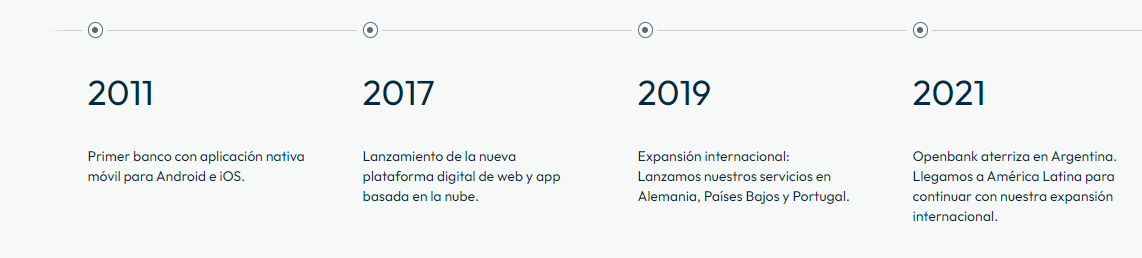
\includegraphics[width=16cm]{historiaopenbank.png}
    \caption{Història OpenBank}
\end{figure}  


